\documentclass{article}

\usepackage{graphicx}
\usepackage{placeins}
\usepackage[utf8]{inputenc}
\usepackage{listings}
\usepackage{hyperref}
\usepackage{xcolor}
\usepackage[nodayofweek,level]{datetime}
\usepackage{ulem}
\usepackage{mathtools}
\usepackage{newfloat}
\DeclareFloatingEnvironment[
    fileext=los,
    listname=List of code snippets,
    name=Snippet,
    placement=tbhp,
    within=none,
]{snippet}

\DeclarePairedDelimiter{\ceil}{\lceil}{\rceil}

\definecolor{darkgreen}{RGB}{50,200,50}
\definecolor{darkcyan}{RGB}{130,230,200}
\definecolor{verylightgray}{gray}{0.85}
\definecolor{goldenbrown}{rgb}{0.558215, 0.0, 0.135316}

\lstdefinelanguage{solidity}
{
	keywords={uint256, bytes32, mapping, address, uint40, bool, uint32, msg, sender, false, true},
	keywordstyle=\color{blue},
	keywords=[2]{pragma, contract, event, enum, struct, function, return, private, public, constant, returns, var, for, !, if, break, continue, throw, &&, ||, else, =, ==, <, >, <=, >=},
	keywordstyle=[2]\color{magenta},
	keywords=[3]{push, pull},	
	keywordstyle=[3]\color{darkcyan},
	comment=[l]{//},
	commentstyle=\color{darkgreen},
	numbers=left,
	extendedchars=false,
	morestring=[b]",
	stringstyle=\color{goldenbrown},
	breaklines=true,
	backgroundcolor=\color{verylightgray},
	basicstyle=\linespread{1}\ttfamily\footnotesize
}

\title{Consensus in declarative process models using distributed smart-contracts}
\author{Mikkel Gaub, \\ Tróndur Høgnason, \\ Malthe Ettrup Kirkbro, \\ \& Mads Frederik Madsen }
\date{}

\begin{document}

\normalem
	\begin{titlepage}
		\maketitle		
		\hspace{-18pt}
		\textit{May 15, 2017}
		\vspace{\fill}
		\section*{Abstract}
		This paper investigates how efficiently declarative process models can be implemented using distributed smart-contracts, more concretely the Dynamic Condition Response (DCR) engine will be implemented on the Ethereum platform, with a focus on minimizing the cost of running such an engine.
		\thispagestyle{empty}
	\end{titlepage}
	\clearpage

	\pagenumbering{arabic}
	\setcounter{page}{1}

	\setcounter{tocdepth}{2}
	\tableofcontents
	\pagebreak

	\section{Introduction}
	In this article we will continue to build upon our previous research with declarative process models on blockchain. 
	In our previous research we have shown how a blockchain can be used to achieve consensus between multiple participants in a declarative process model, and we built a proof of work declarative workflow management system (WfMS) that utilized Bitcoins blockchain to achieve consensus.
 
	We found Bitcoins blockchain to be restrictive which is understandable, as it is not intended for anything else than a ledger of transaction for the cryptocurrency Bitcoin. 
	But the underlying technology, the blockchain, has been used in many other applications and platforms. 
	We will implement a WfMS using a Dynamic Condition Response (DCR) engine on one of these platforms, namely Ethereum.
	Since everything costs money in Ethereum, optimization is key in order for a solution to be viable.
	Ethereum is also a very new technology and is constantly subject to change, making it fairly undocumented aside from the yellow- and whitepaper.
	We will therefore be experimenting with several different system structures and comparing their costs in order to find the best solution.

	With the growing interest in decentralization in computer science we think it is of the utmost importance to continue to explore and improve upon existing decentralization techniques.

	\subsection{Previous work}
	Our previous work with blockchains was done for our bachelor thesis \cite{bachelor}. 
	The main idea we will carry on from our bachelor thesis is that a blockchain can be used to create a consensus protocol. 
	We will therefore not go into great detail of how we can achieve consensus with a blockchain. 
	The following section will provide the information we deem necessary to understand how we can achieve consensus with a blockchain, but no literature to support this. 
	Interested parties can review the previously mentioned thesis in which there is references to a great deal of literature to support this claim.
	\subsubsection{Achieving consensus with blockchains}

	\subsubsection{Motivation to use Ethereum}
	The previous DCR engine we built utilized Bitcoins blockchain to validate workflow creation and execution attempts by storing the hash of these on the blockchain.
	The actual verification of the legality of executions with respect to DCR logic and execution rights was done on a DCR engine running locally on a users machine.
	Thus our application relied heavily on the majority of users involved in a workflow were actually using our DCR engine to verify the legality of executions. 

	Our previous DCR engine made it infeasible for an adversary to fake executions or claim that executions were part of another workflow than what benevolent users thought.
	Instead it was vulnerable to loss of local data. 
	
	If a user managed to remove all local traces of a workflow, it could be difficult to claim that the traces of executions belonged to a certain workflow and therefore hard to prove that a user actually did execute some specific activity. Furthermore reconstruction of a lost workflow would be nigh impossible without access to another copy of the workflow.

	Ethereums blockchain has other possibilities, as one is able to verify \textbf{1)} the existence of specific source code on the blockchain \textbf{2)} if code on the blockchain has been run \textbf{3)} if the code was run successfully or not.
	Any user participating in a workflow using a DCR engine running on Ethereums blockchain can therefore be sure\footnote{Quite sure...ref til vulnerabilities} that the source code is unchanged and that every execution is validated with respect to both DCR logic and execution rights in the same way Bitcoins blockchain verified workflow creation and execution attempts.

	\section{Dynamic Condition Response graphs}
	\label{sec:dcr-graphs}
	A DCR graph is a representation of a workflow.
	The graph is made up of one or more activities with zero or more relations between them. 
	The following section is loosely based on a similar description in our bachelor's thesis \cite{bachelor}. 

	\subsection{Activity}
	The activities in a DCR graph have three attributes: included, executed and pending. 
	The attributes can be true or false. 
	Furthermore an activity can have role and actor specific execution rights.

	\subsubsection{Included attribute}
	If the include attribute of an activity is true, the activity is included and it can be executed. 
	If the attribute is false, the activity is excluded and can no longer be executed.

	\subsubsection{Pending attribute}
	If any activity in a workflow has a pending attribute that is true and the activity is included, the workflow is in an unfinished state.
	Every time an activity is executed its pending attribute is set to false.
	This means that setting the pending attribute of an included activity to true is specifying that this activity must be executed or excluded at some point to leave the workflow in a finished state.

	\subsubsection{Executed attribute}
	If an activities executed attribute is false executing the activity will set its executed attribute to true.
	Executing an already executed activity will have no effect on the executed attribute.

	\begin{figure}[!ht]
		\centering
		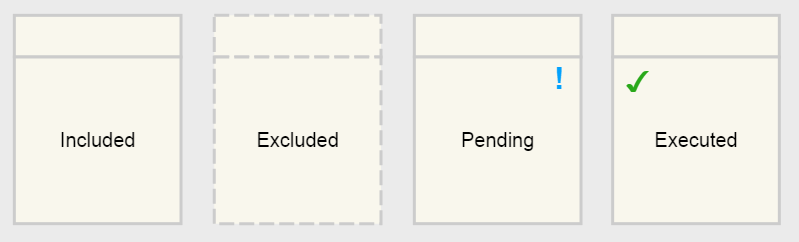
\includegraphics[width=1\textwidth]{figures/activity_states.png}
	 	\caption[Activity States]
	 	{From left to right: A visual representation of an included, excluded, pending and executed activity as presented on \href{http://www.dcrgraphs.net}{dcrgraphs.net}}.
	\end{figure}

	\subsection{Relations}
	There are five types of relations which define different types of relationships between activities in a workflow. 
	These five are the \emph{condition}, \emph{response}, \emph{include}, \emph{exclude} and \emph{milestone} relations.

	\subsubsection{Condition relation}
	If there is a condition relation from activity A to activity B, then B can only be executed if A's executed attribute is true or A is excluded.
	\begin{figure}[!ht]
		\centering
		
\includegraphics[width=0.3\textwidth]{figures/ConditionRelation.png}
	 	\caption[Condition relation]
	 	{Condition relation}
	\end{figure}

	\subsubsection{Response relation}
	If there is a response relation from activity A to activity B, then B's pending attribute will be set to true every time A is executed.
	\begin{figure}[!ht]
		\centering
		
\includegraphics[width=0.3\textwidth]{figures/ResponseRelation.png}
	 	\caption[Response relation]
	 	{Response relation}
	\end{figure}

	\subsubsection{Include relation}
	If there is an include relation from activity A to activity B, then B's included attribute will be set to true every time A is executed.
	\begin{figure}[!ht]
		\centering
		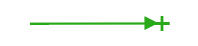
\includegraphics[width=0.3\textwidth]{figures/IncludeRelation.png}
	 	\caption[Include relation]
	 	{Include relation}
	\end{figure}

	\subsubsection{Exclude relation}
	If there is an exclude relation from activity A to activity B, then B's included attribute will be set to false every time A is executed.
	\begin{figure}[!ht]
		\centering
		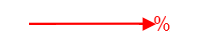
\includegraphics[width=0.3\textwidth]{figures/ExcludeRelation.png}
	 	\caption[Exclude relation]
	 	{Exclude relation}
	\end{figure}

	\paragraph{Milestone relation}
	If there is a milestone relation from activity A to activity B, then B can only be executed if A's pending attribute is false or A's included attribute is false.
	\begin{figure}[!ht]
		\centering
		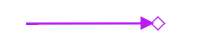
\includegraphics[width=0.3\textwidth]{figures/MilestoneRelation.png}
	 	\caption[Milestone relation]
	 	{Milestone relation}
	\end{figure}

	\subsection{Example workflow}
	Figure \ref{fig:exampleWorkflow} shows an DCR graph modeling a support ticket workflow. When the workflow is created only \texttt{Submit ticket} is executable. 
	\texttt{Close ticket} cannot be executed as it is excluded and there is a condition relation to it from an activity that is not executed. 
	\texttt{Propose solution} and \texttt{Reject solution} cannot be executed as there are condition relations to them from activities that have not been executed. 
	Lastly \texttt{Accept solution} cannot be executed as there is a milestone relation to it from \texttt{Propose solution} which is pending and not excluded.
	\begin{figure}[!ht]
		\centering
		\includegraphics[width=\textwidth]{figures/exampleWorkflow.png}
	 	\caption[Example workflow]
	 	{Example workflow}
	 	\label{fig:exampleWorkflow}
	\end{figure}
	\FloatBarrier
	A typical example of an execution order of the example workflow would look like this:
	\begin{enumerate}
		\item The customer executes \texttt{Submit ticket} which excludes itself. 
		This includes \texttt{Close ticket}, but \texttt{Close ticket} is still not executable, as there is a condition relation to it from \texttt{Accept solution}.
		\texttt{Propose solution} however is now executable.
		\item The supporter executes \texttt{Propose solution}. Now \texttt{Accept solution} is executable as \texttt{Propose solution} is no longer pending and \texttt{Reject solution} is also executable as \texttt{Propose solution} is executed. 
		Furthermore \texttt{Accept solution} is now pending and must therefore be executed or excluded at some point.
		\item If the customer is not satisfied with the solution he can execute \texttt{Reject solution} which will prevent execution of \texttt{Accept solution}, as \texttt{Propose solution} is now pending and still included. 
		The workflow is now in the same state as in step 2 except from the fact that \texttt{Reject solution} is executable. 
		Executing \texttt{Reject solution} will however have no effect, as \texttt{Propose solution} is already pending.
		\item If the customer on the other hand is satisfied with the supporters solution he can execute \texttt{Accept solution}.
		Executing \texttt{Accept solution} will exclude \texttt{Propose solution} and \texttt{Reject solution}.
		This leaves \texttt{Close ticket} executable and pending.
		To leave the workflow in a finished state the supporter must execute \texttt{Close ticket}. 
	\end{enumerate}

	\section{Ethereum}
	In order to implement the DCR engine as a distributed smart-contract, we use the platform Ethereum. 
	Ethereum is a blockchain technology that allows for code publication and execution via the Ethereum blockchain.  
	Central for blockchain technologies is a cryptocurrency, which is used to provide incentive for mining and to pay for the verification and computation of the published code.
	Ethereum's cryptocurrency is called \emph{Ether}.
	As an intermediary currency, the stack codes of the Ethereum Virtual Machine (EVM) have a value associated with it in a unit called gas, see appendix \ref{app:gas-prices}, which is then payed for with Ether by the person publishing that code.
	The EVM is, in the words of the creators of Ethereum, a "quasi-Turing-completeness"\cite{yellow-paper}.
	This is explained in that even if the gas is given away for free, there will be a structural limit in that unlimited gas is not representable.

		\subsection{Currency}
		The currency of Ethereum is called Ether, and mining a block has a base reward of five Ether.
		Additional rewards given for blocks which include uncles (see the following section). 
		Lastly a miner also gets a reward based on how much computation power is needed to run the code included in a block. 
		The last reward is essentially equivalent to the transaction fees in Bitcoin.

		To store data or run code on the Ethereum platform one has to spend an amount of gas. 
		All computations have a set gas cost and can be seen in appendix \ref{app:gas-prices}, and Ethereum provides tools to calculate how much gas a proposed execution some code would cost.
		Gas has no inherent value, but instead a user has to specify how much Ether he wants to spend per gas. 
		The user then specifies how much gas he wants to send with the execution request and how much Ether he is willing to spend per gas. If the user has set the price he is willing to pay per gas to low, no miner will to include the users code execution in his block.
		If on the other hand miners set their minimum price for inclusion to high, no one is willing to use Ethereum. 
		The price per gas is therefore based on the principle of supply and demand, where the commodity is computation power.

		If a user send to little gas to complete the computations he requested, the requested computations are rolled back as if they never happened. 
		The used gas is not returned to the user. 
		This is a security feature of Ethereum that prevents denial of service attacks by requesting many computationally heavy transactions without having the means to pay for them. 
		This feature is also what makes Ethereum "quasi-Turing-complete" and not Turing complete.

		\subsection{Blockchain}
		A blockchain is a distributed and decentralized database, consisting of blocks\cite{bitcoin-white-paper}. 
		Each block contains the changes to the database since the last block, as well as a reference to the block preceding it, thereby forming a chain.
		To ensure that data cannot be overwritten, each block must be verified by a cryptographic puzzle, namely finding a nonce, a proof-of-work, to include in the block such that the hash of the block information is below a variable threshold, called the difficulty\cite{bitcoin-white-paper}. 
		The process of finding a correct nonce is commonly called mining.
		The difficulty is automatically adjusted according to the the frequency of mined blocks in relation to the desired frequency.
		Multiple blocks can be published simultaneously, and therefore reference the same preceding block. This situation is called a fork and is normally solved when one of the two chains has is longer than the other(s).

		The specification of Ethereum's blockchain\cite{yellow-paper, ethereum-white-paper} contain some interesting features, which makes it different it from most other blockchain technologies.
		
		Finding a proof-of-work in Bitcoin consists of incrementing the nonce and hashing the block header to check if it fulfills the difficulty requirements. 
		This is purely a question of computational power and has spawned a market for hardware specifically adapted to hashing, giving it an advantage compared to the standard processing units of a generic user. 
		As this hardware is fairly expensive, this favors the so called mining pools, which are large numbers of machines combining their computational power in order to find a proof-of-work and thereafter sharing the reward for mining a block. 
		This specialization undermines the decentralized aspect of the blockchain and in order to eliminate it, the proof-of-work in Ethereum is bound by memory, because checking the hash involves creating a large directed graph and thereafter checking the values of a number of leaf-nodes as specified by an interpretation of the nonce. 
		The creators of Ethereum estimate that any significant progress in the performance of memory would be relatively cheap and useful in many more situations than just in the mining of Ethereum blocks, as opposed to the hardware used for mining in Bitcoin.

		In Bitcoin miners are rewarded by themselves when they mine the block, as they are allowed to include a transaction of a set amount of bitcoins to themselves.
		This is very similar to how Ethereum miners are rewarded, however they are additionally rewarded for including blocks that are not included in the longest chain.
		These are called uncles or ommers and are included in order to not have miners waste computational power, which would result in attackers potentially needing less than the majority of the network in order to overtake the current longest chain. 
		The transactions contained in the uncles are ignored, as they could contain information conflicting with the contents of the blocks in the chain, but they are still included in the accumulated difficulty of the chain. Contrary to Bitcoins blockchain, where forks are resolved by choosing the longest chain, forks on Ethereums blockchain are solved by choosing the chain with the highest accumulated difficulty.
		Both the miners of the uncle and the miner who includes the uncle are rewarded in this system, with a fraction of the reward for mining a block contained in the main blockchain, ensuring incentive for miners to make the chain as heavy, difficulty-wise, as possible but still prioritizing mining new blocks.

		Aside from having to manage the balance of a users account, the blockchain of Ethereum also has the ability to store user-created code encapsulated in so called contracts. All users can interact with code on the blockchain, given that they can pay for the execution of said code. 
		When a transaction is included in a block, part of the verification of that block is running the code specified by the transaction and making sure that the state of the contract(s) affected by the transaction is mutated accordingly.

		Since this means that anyone attempting to verify a block needs to run arbitrary code, the allowed operations need to be very carefully formulated and vetted. 
		This has led the creators of Ethereum to create their own virtual machine, namely the Ethereum Virtual Machine (EVM). 

		\subsection{Ethereum Virtual Machine}	
		Due to the unique environment in which the EVM is used, there are equally unique constraints in the EVM:
		\begin{description}
			\item [Max stack size and limited stack access] The stack is limited to 1024 elements and COPY and SWAP operations can only access the top 16 elements of the stack. This infers some limitations on the number of parameters which can be given to a function.
			\item [No libraries] External functions are limited to what other contracts offer.  
			\item [No types] The EVM only operates in words of 32-byte Big Endian integers, meaning no floating point operations exist.
			\item [No true randoms] As part of block verification is ensuring that the state of a contract corresponds to the result of the functions performed on it, code needs to be deterministic and there are therefore no true random numbers.
			\item [Contract data access] All contracts are sandboxed inside their own environment, meaning that they cannot access the data of other contracts, except by calling their functions.
		\end{description}

		\subsubsection{Programming languages}
		There is a large number of options for programming languages which can compile to EVM bytecode, but due to Ethereum being a relatively new invention it is still subject to frequent low-level changes. 
		Most languages which can be compiled to EVM stack code are therefore languages specifically designed for Ethereum.
		Some of the languages implemented for Ethereum are Solidity, Viper, Serpent, LLL and Mutan which all are very basic at the moment, but the languages are all in active development, except for Mutan.

		We have chosen to implement our solutions in Solidity as it seems most mature of the listed options, at the time of writing.

	\section{Implementation requirements}
	\label{sec:implementation-requirements}
	The data structure of the two implementation will be as follows:

	\begin{description}
		\item[Workflow] The workflow must contain a name, a list of activities and a list of access rights.
		\item[Activity] Each activity must contain a name, a list of the relations related to it and a list of users who are allowed to execute it.
		\item[Relations] The five relations described in Section \ref{sec:dcr-graphs} must be supported. They should be implemented in two categories:
			\begin{enumerate}
				\item Incoming: The relations in this category are the \emph{milestone} and \emph{condition}. These relations specify which other activities have \emph{milestone} or \emph{condition} relations to the activity containing the relations. Those activities' attributes must be checked to ensure the activity containing the relation can be executed.
				\item Outgoing: The relations in this category are the \emph{response}, \emph{exclude} and \emph{include} relation. These relations specify which activities' attributes must be updated after an execution on the activity containing the relation. 
			\end{enumerate}
		\item[Access rights] Should be indicated by the public key of a given user.
	\end{description}

	In order to ensure that the two implementations can be properly compared, they will support, and initially be limited to, the following functionality: 
	
	\begin{description}
		\item[Workflow creation] The implementations must support the creation of a workflow. Workflow creation should be performed with a single method call and must be atomic, meaning that no workflow can be partially created. This also means that no workflow can be modified past its creation.
		\item[Execution attempts] It must be possible to attempt to execute any activity at any time.
		\item[Activity execution] If an activity is executable following DCR logic, it must be executed if a user with the necessary rights requests an execution of it. The execution must also update the attributes of any other activities as prescribed by the outgoing relations it has.
		\item[Contract suicide] Any created contract must be allowed to self-destruct, when called by the creating user.
		\item[Data retrieval] The data stored must be accessible by any authorized user.
	\end{description}

	\section{Multi-contract implementation}
	% Design decisions
	The first implementation approach, is creating an Ethereum contract for each workflow, called the Multi-contract implementation (since multiple workflows will multiple contracts). 
	The contract contains the data for exactly one workflow, i.e. the workflow's name, the list of activities in the workflow etc, as well as the data of all the activities in the workflow as well as their relations. 
	Furthermore each contract will contain functions to support the functionality described in section \ref{sec:implementation-requirements}.

	This approach strikes a middle ground between the modularity obtained from having each self contained data structure, i.e. the activities and/or the relations being published as separate contracts, and the efficiency obtained from having multiple entire workflows published in a single contract. 
	The multi-contract implementation achieves a relatively high cohesion as all data relevant to a single workflow is contained in a single contract, while reducing the coupling between contracts, since no external function calls are necessary to achieve the required functionality.

		%Relatively expensive in theory - include?

	% Important implementation details
		%Data structure
		\subsection{Implementation details}
		The data structures in the Multi-contract implementation are relatively simple.
		Only a single struct is defined, used to represent an activity.
		The entire contract is the workflow, so no explicit data structure is need for the workflow, instead the contract's fields contain the relevant data for the workflow.
		The contract contains a \texttt{bytes32 name} field representing the workflow's name, an array of activities and the Ethereum address of the creating account.
		\begin{snippet}[!ht]
			\centering
			\begin{lstlisting}[language=solidity, numbers=none]
struct Activity {
    // State
    bytes32 name;
    bool included;
    bool executed;
    bool pending;

    // Outgoing relations:
    uint32[] include;
    uint32[] exclude;
    uint32[] response;
    
    // Incoming relations:
    uint32[] condition;
    uint32[] milestone;

    // Access rights:
    address[] whitelist;
}				
			\end{lstlisting}
		 	\caption[The \texttt{Activity} struct]
		 	{The \texttt{Activity} struct}
		 	\label{sni:activity-struct}
		\end{snippet}
		The \texttt{Activity} struct (see snippet \ref{sni:activity-struct}) is made up a \texttt{bytes32} name, three booleans representing the activity's attributes, a list for each relation type and a list for containing the Ethereum addresses that are allowed to execute the activity.

		%Construction
		The entire workflow is initialized on contract construction. 
		Since the Solidity language currently (v. 0.4.10) does not support neither structs nor nested arrays as parameters in contract construction, the workflow construction is a bit complicated. 

				\begin{snippet}[!ht]
			\centering
			\begin{lstlisting}[language=solidity, numbers=none]
// We expect the 'relations' array is formed such that the first index is the FROM activity and the next index is the TO activity. Rinse and repeat.
for(i = 0; i < relations.length; i=i+2){
    if(relationType[i/2] == RelationType.Include)        	activities[relations[i]].include.push(relations[i+1]);
    else if(relationType[i/2] == RelationType.Exclude)   	activities[relations[i]].exclude.push(relations[i+1]);
    else if(relationType[i/2] == RelationType.Response)  	activities[relations[i]].response.push(relations[i+1]);
    else if(relationType[i/2] == RelationType.Condition) 	activities[relations[i+1]].condition.push(relations[i]);
    else if(relationType[i/2] == RelationType.Milestone) 	activities[relations[i+1]].milestone.push(relations[i]);
    else throw;
}			
			\end{lstlisting}
		 	\caption[Mapping relations to activities in the multi-contract construction]
		 	{Mapping relations to activities in the multi-contract construction}
		 	\label{sni:relation-mapping}
		\end{snippet}

		For instance, every relation in the workflow is represented in a single \texttt{uint32} list in the constructor, called \texttt{relations}. 
		To map these to activities (see snippet \ref{sni:relation-mapping}), the structure of the relations-array have to uphold the invariant that, for an even \texttt{i}, \texttt{relations[i]} is the id of the activity the relation is coming from, and \texttt{relations[i+1]} is the id of the activity the relation is going to.

		Excluding contract construction, the rest of the functions are reasonably straight forward.
		The code for the Multi-contract implementation can be found in its entirety in appendix \ref{app:multi-contract-code}.



	% How it runs missing

	\section{Mono-contract implementation}
	The idea behind the second implementation is that the gas costs of Ethereum are largely dominated by the price of creating a contract. If we observe appendix \ref{app:gas-prices} we find that the most expensive operation is the contract creation operation $G_{create}$ which costs 32000 gas. 
	This incentiveses us to create as few contracts as possible. 

	The second implementation is therefore a single contract with all workflows. 
	Workflows that are created are stored in a workflow array. 
	The methods of the Mono-contract implementation are largely the same as in the Multi-contract implementation. 
	The key difference is that the methods must access an index of the workflow array to retrieve the specified array before beginning modification of a workflow.

	The limitations of Solidity are clearly reflected in the \texttt{createWorkflow} method which creates a workflow. 
	Because of the limit on number of bytes the EVM can go back, the number of variables a method can take is limited. 
	This limitation creates problems for methods which require large amount of different data. 
	Some of the compromises we have made to limit the number of variables in the \texttt{createWorkflow} are listed below:
	\begin{enumerate}
		\item A byte array is used to represent all names relevant to the workflow. The first index is used for the workflow name, indexes 1-32 are used for group names and indexes 33-$n$ ($n = number \quad of \quad activities - 33$) are used for activity names.
		\item Instead of three boolean list representing the attributes of the activities, the array \texttt{activityStates} of size three of boolean arrays is used.
		\item An array of size three of unsigned integer arrays is used to represent activity data. 
		\begin{enumerate}
			\item The first array is used as a counter for how many relations will be stored on each activity. We use this counter as there is only one array containing the type of the relation and one array containing the id of the activity the relation should point to. But there is nothing indicating which activity the relation should be stored on.
			\item The second array is used to represent the number of public keys that are authorized to execute an activity. This counter is used as there is only a single list with all authorized user, but there is nothing associating them with any specific activity.
			\item The last array is used to represent the number of groups that are authorized to execute an activity. This is done for the same reasons as above; there is only one list with group authorizations.
		\end{enumerate}
	\end{enumerate}

	\section{Comparison}
	In order to compare the solutions to each other, a simple workflow has been created modeling each of the five relations...

	\begin{description}
		\item[Contract creation]
		\item[Successful execution] ...
		\item[Failed execution] ... 
	\end{description}

	\section{Optimizations}

		\subsection{Bitfields}

	\section{Discussion}

	\section{Further features}
		As the optimized solution is a completely bare-bones implementation of the DCR engine, there are multiple potential expansions of the functionality and features which could be implemented on top of the current structure, both with regards to the functionality supported by DCR and by Ethereum.
		These features would be fairly use-case dependent and since they would probably have an effect on the cost of running a workflow where those features are not even used, they should only be implemented in instances where they would actually be used.

		\subsection{Workflow changes}
		\label{sec:workflow-changes}

		In a case where a companies definition of a workflow changes, but the history of the current workflow is still relevant in the context of the new, it could be beneficial to simply change the workflow according to the specifications of the new.
		This poses some challenges in the way that the workflow might change its definition, subtly or drastically, as covered in \cite{hierarchical-declarative-modelling} with regards to refinement.
		A verification of any given change to a workflow, as specified in the article, would be risky to implement in Ethereum, as it is a computationally very hard problem and a user would be hard pressed to pay for it.
		Therefore a different method of verification would probably be more viable, for example by disallowing certain types of conditions.
		Verification could also be foregone in the favor of the simple method of requiring the user proposing the change to be authorized to change both workflows. 

			\subsubsection{Vulnerabilities}

		\subsection{External relations}
		\label{sec:external-relations}
		In the proposed solutions, workflows are viewed as completely separate from each other. 
		This means that if a connection between the two is desired, it would require the entire workflow to be duplicated per other workflow relevant to it.
		An alternative to this, could be to create external relations between the workflows, as described in \cite{distributed-workflows}, given that the user creating the relations has some sort of ownership of both workflows.

		But great care would be needed when allowing external contracts to create incoming relations to a workflow, as incoming relations can make workflows less restrictive, which is related to the issues outlined with regards to workflow changes (See section \ref{sec:workflow-changes}). 
		An example of this is an exclude relation from an activity $A_{ex}$ in an external workflow to an activity $B$ with a condition relation to another activity $C$ in the original workflow. 
		Executing $A_{ex}$ would exclude $B$ and activity $C$ would be executable without executing $B$ as intended when constructing the condition relation.

		An implementation of this in the mono-contract solution would be fairly simple, as well as cheap, as all the workflows are potentially stored in a single contract.

			\subsubsection{Vulnerabilities}

		\subsection{External contract conditions}

		As the public methods of a contract on the Ethereum blockchain is accessible by other contracts, provided they are called correctly and with sufficient funds, it would be possible to construct a workflow where some activities are dependent on the values of other contracts.
		These dependencies could be to all sorts of sources, as long as they are trusted by the creator of the workflow. 
		An example could be a contract showing the value of currencies or perhaps a contract producing synchronized random numbers.

		In the case where each company has their own mono-contract, possibly due to their diverse needs for specific features, or the case where a multi-contract solution is used, this functionality would be closely tied to the functionality of external relations (See section \ref{sec:external-relations}).

			\subsubsection{Vulnerabilities}

	\section{Conclusion}

	\pagebreak
	\addcontentsline{toc}{section}{References}	
	\bibliographystyle{plain}
	\begin{thebibliography}{99}

		\bibitem{yellow-paper}
		Wood, G.
		\textit{Ethereum: A Secure Decentralised Generalised Transaction Ledger}. 
		\url{http://yellowpaper.io}.
		Accessed 2017-05-09.

		\bibitem{bachelor}
		Gaub et al.
		\textit{Consensus in peer-to-peer systems}.
		Unpublished manuscript.
		IT-University of Copenhagen,
		Denmark,
		2016.

		\bibitem{ethereum-white-paper}
		Various authors.
		\textit{White Paper}.
		\url{https://github.com/ethereum/wiki/wiki/White-Paper},
		Accessed 2017-05-09.

		\bibitem{bitcoin-white-paper}
		Nakamoto, S.
		\textit{Bitcoin: A Peer-to-Peer Electronic Cash System}.
		\url{https://bitcoin.org/bitcoin.pdf},
		Accessed 2017-05-09.

		\bibitem{distributed-workflows}
		Hildebrandt, T., Mukkamala, R., and  Slaats, T.
		\textit{Safe Distribution of Declarative Processes}.
		\url{https://pure.itu.dk/ws/files/34548793/paper_5.pdf},
		Accessed 2017-05-10.

		\bibitem{hierarchical-declarative-modelling}
		Debois, S., Hildebrandt, T., Slaats, T.
		\textit{Hierarchical Declarative Modelling with Refinement and Sub-processes}.
		\url{asd},
		Accessed 2017-05-11

	\end{thebibliography}

	\clearpage

	\addcontentsline{toc}{part}{Appendices}	

	\appendix

	\section{Gas prices}
		\label{app:gas-prices}

		As of May 9th, 2017, the gas prices are \cite{yellow-paper}: 
		\begin{table}[!ht]
		\footnotesize
		\noindent \begin{tabular}{| l | l | p{8cm} |}
			\hline
			Name 				& Value 	& Description \\ \hline
			$G_{zero}$ 			& 0 		& Nothing paid for operations of set $W_{zero}$. \\ \hline
			$G_{base}$ 			& 2 		& Amount of gas to pay for operations of the set $W_{base}$. \\ \hline
			$G_{verylow}$ 		& 3 		& Amount of gas to pay for operations of the set $W_{verylow}$. \\ \hline
			$G_{low}$ 			& 5 		& Amount of gas to pay for operations of the set $W_{low}$. \\ \hline
			$G_{mid}$ 			& 8 		& Amount of gas to pay for operations of the set $W_{mid}$. \\ \hline
			$G_{high}$ 			& 10 		& Amount of gas to pay for operations of the set $W_{high}$. \\ \hline
			$G_{extcode}$ 		& 700 		& Amount of gas to pay for operations of the set $W_{extcode}$. \\ \hline
			$G_{balance}$ 		& 400 		& Amount of gas to pay for a BALANCE operation. \\ \hline
			$G_{sload}$ 		& 200 		& Paid for a SLOAD operation. \\ \hline
			$G_{jumpdest}$ 		& 1 		& Paid for a JUMPDEST operation. \\ \hline
			$G_{sset}$ 			& 20000 	& Paid for an SSTORE operation when the storage value is set to non-zero from zero. \\ \hline
			$G_{sreset}$ 		& 5000 		& Paid for an SSTORE operation when the storage value's zeroness remains unchanged or is set to zero. \\ \hline
			$R_{sclear}$ 		& 15000		& Refund given (added into refund counter) when the storage value is set to zero from non-zero. \\ \hline
			$R_{suicide}$ 		& 24000 	& Refund given (added into refund counter) for suiciding an account. \\ \hline
			$G_{suicide}$ 		& 5000 		& Amount of gas to pay for a SUICIDE operation. \\ \hline
			$G_{create}$ 		& 32000		& Paid for a CREATE operation. \\ \hline
			$G_{codedeposit}$ 	& 200 		& Paid per byte for a CREATE operation to succeed in placing code into state. \\ \hline
			$G_{call}$ 			& 700		& Paid for a CALL operation. \\ \hline
			$G_{callvalue}$ 	& 9000		& Paid for a non-zero value transfer as part of the CALL operation. \\ \hline
			$G_{calstipend}$ 	& 2300		& A stipend for the called contract subtracted from $G_{callvalue}$ for a non-zero value transfer. \\ \hline
			$G_{newaccount}$ 	& 25000		& Paid for a CALL or SUICIDE operation which creates an account. \\ \hline
			$G_{exp}$ 			& 10 		& Partial payment for an EXP operation \\ \hline
			$G_{expbyte}$ 		& 10		& Partial payment when multiplied by $\ceil{log_{256}(exponent)}$  for the EXP operation. 	 \\ \hline
			$G_{memory}$ 		& 3			& Paid for every additional word when expanding memory. \\ \hline
			$G_{txcreate}$ 		& 32000		& Paid by all contract-creating transactions after the Homestead transition. \\ \hline
			$G_{txdatazero}$ 	& 4 		& Paid for every zero byte of data or code for a transaction. \\ \hline
			$G_{txdatanonzero}$ & 68		& Paid for every non-zero byte of data or code for a transaction. \\ \hline
			$G_{transaction}$ 	& 21000		& Paid for every transaction. \\ \hline
			$G_{log}$ 			& 375 		& Partial payment for a LOG operation. \\ \hline
			$G_{logdata}$ 		& 8			& Paid for each byte in a LOG operation's data. \\ \hline
			$G_{logtopic}$ 		& 375		& Paid for each topic of a LOG operation. \\ \hline
			$G_{sha3}$ 			& 30		& Paid for each SHA3 operation. \\ \hline
			$G_{sha3word}$ 		& 6			& Paid for each word (rounded up) for input data to a SHA3 operation. \\ \hline
			$G_{copy}$ 			& 3			& Partial payment for *COPY operations, multiplied by words copied, rounded up. \\ \hline
			$G_{blockhash}$ 	& 20		& Payment for BLOCKHASH operation. \\ 
			\hline
		\end{tabular}
		\end{table}
		\FloatBarrier

		\subsection{Instruction sets}
		\begin{description}
			\item[$W_{zero}$] = \{STOP, RETURN\}
			\item[$W_{base}$] = \{ADDRESS, ORIGIN, CALLER, CALLVALUE, CALLDATASIZE, CODESIZE, GASPRICE, COINBASE, TIMESTAMP, NUMBER, DIFFICULTY, GASLIMIT, POP, PC, MSIZE, GAS \}
			\item[$W_{verylow}$] = \{ADD, SUB, NOT, LT, GT, SLT, SGT, EQ, ISZERO, AND, OR, XOR, BYTE, CALLDATALOAD, MLOAD, MSTORE, MSTORES, PUSH*, DUP*, SWAP*\}
			\item[$W_{low}$] = \{MUL, DIV, SDIV, MOD, SMOD, SIGNEXTEND\}
			\item[$W_{mid}$] = \{ADDMOD, MULMOD, JUMP\}
			\item[$W_{high}$] = \{JUMPI\}
			\item[$W_{extcode}$] = \{EXTCODESIZE\}			
		\end{description}

	\section{Test workflow}

		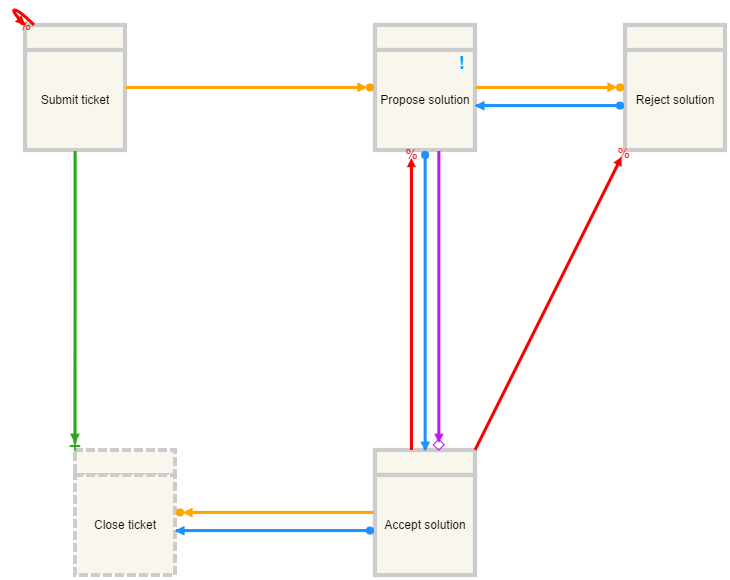
\includegraphics[scale=0.45]{figures/ExampleWorkflow.png}

	\section{Multi-contract}

		\subsection{Code}
		\label{app:multi-contract-code}

			\lstinputlisting[language=solidity]{../contracts/workflow.sol}

		\subsection{Costs}

			\begin{tabular}{| l | l |}
				\hline
				Action & Cost (gas) \\ \hline
				Contract creation & 0 \\
				\hline
			\end{tabular}

	\section{Mono-contract}

		\subsection{Code}

			\lstinputlisting[language=solidity]{../contracts/monolith.sol}

		\subsection{Costs}

			\begin{tabular}{| l | l |}
				\hline
				Action & Cost (gas) \\ \hline
				Contract creation & 0 \\
				\hline
			\end{tabular}

\end{document}